\documentclass{article}
\usepackage[utf8]{inputenc}
\usepackage{enumitem}
\usepackage{amsmath}
\usepackage{mathtools}
\usepackage{amsfonts}
\DeclarePairedDelimiter\ceil{\lceil}{\rceil}
\DeclarePairedDelimiter\floor{\lfloor}{\rfloor}
\newcommand*\xor{\mathbin{\oplus}}
\usepackage[table,xcdraw]{xcolor}
\usepackage{graphicx}
\usepackage{float}
\usepackage{amssymb}
\usepackage{adjustbox}
\usepackage{caption}
\usepackage{subcaption}
\usepackage[a4paper,margin=1in,footskip=0.25in]{geometry}
\newcommand{\xmod}[1]{\left(\bmod\ #1\right)}
\newcommand{\ximplies}{\Rightarrow\,}
\newcommand{\ncproblem}[1]{\subsection*{Problem #1}}
\newcommand{\problem}[1]{\clearpage\subsection*{Problem #1}}
\newcommand{\xbf}[1]{\mathbf{#1}}
\newcommand{\xbb}[1]{\mathbb{#1}}
\newcommand{\oa}[1]{\overrightarrow{#1}}
\newcommand{\pd}[1]{\frac{\partial}{\partial #1}}

\title{\huge{Generative Adversarial Urban Growth Prediction of Doha}}
\author{Ziad Khattab}
\date{}

\begin{document}

\maketitle

\section{Purpose}
This project's objective is to create an artificial neural network that can predict the urban coverage of Doha over time. To accomplish this, the network should take a sequence of satellite images, such as the following: 

\begin{figure}[H]
    \caption{satellite images of Doha in 2006 (left) vs. 2016 (right)}
    \centering
    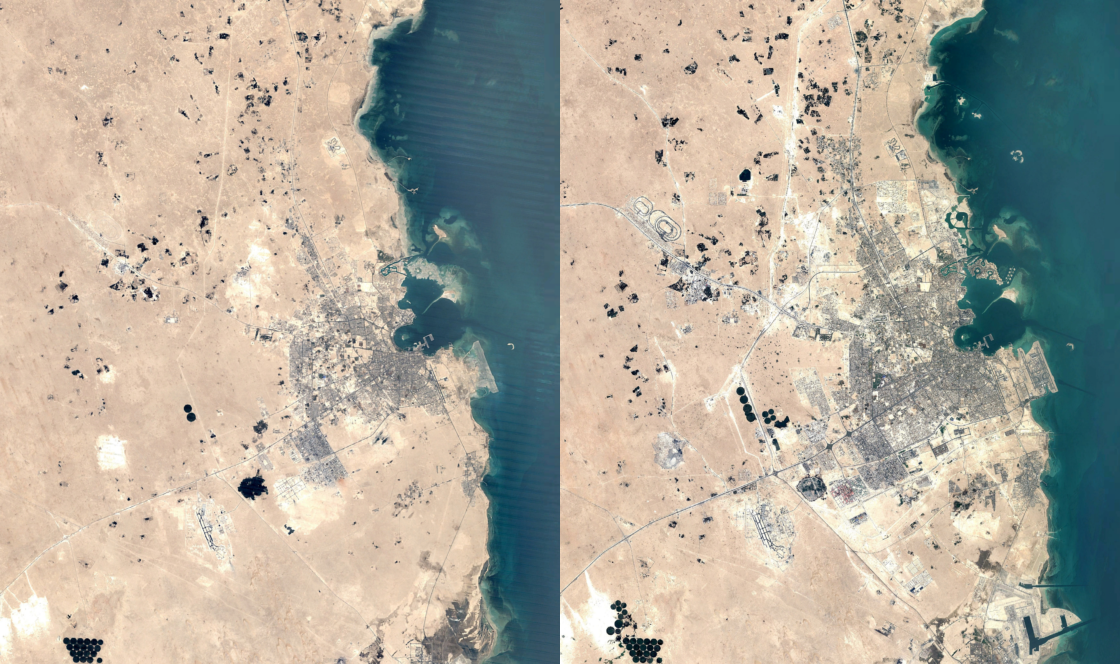
\includegraphics[width=0.7\linewidth]{2006-2016-comp.png}
\end{figure}

and generate simulated satellite maps of what Doha will look like in the future that meet the following requirements:
\begin{enumerate}[label=(\alph*)]
    \item Display an image of a simulated Doha that preserves both image quality and accuracy, as defined by multiple loss functions and metrics (refer to subsections 2.3-2.4). 
    \item Preserve the coastline and water elements virtually unchanged.
\end{enumerate}

\clearpage

\section{Process}

\subsection{Network model}

We want to be able to generate images that can predict Doha's growth up to 2035, using a model trained on yearly images of Doha from 2010-2020. This requires not only the identification of growth patterns, but the ability to generate images of future maps with decently realistic quality and good enough definition to visually identify urban and non-urban areas. For this, a generative adversarial network (GAN) is used. \cite{goodfellow}

In a GAN, a generator network receives the history frames and attempts to provide a realistic continuation to the clip, and a discriminator network attempts to determine whether the clips it receives are real or fake, assigning a probability to the image between 0 and 1 of how likely it is to be real. The two networks compete against one another, with the generator attempting to fool the discriminator into thinking that the generated output images are areal, while the discriminator attempts to pick apart real and fake images more accurately.

We chose to use a GAN as opposed to other models that could generate predicted images, such as a recurrent neural network (RNN), due to GANs' comparative strength in predictions over long time frames.  

\begin{figure}[H]
    \caption{graph of the generative adversarial model}
    \centering
    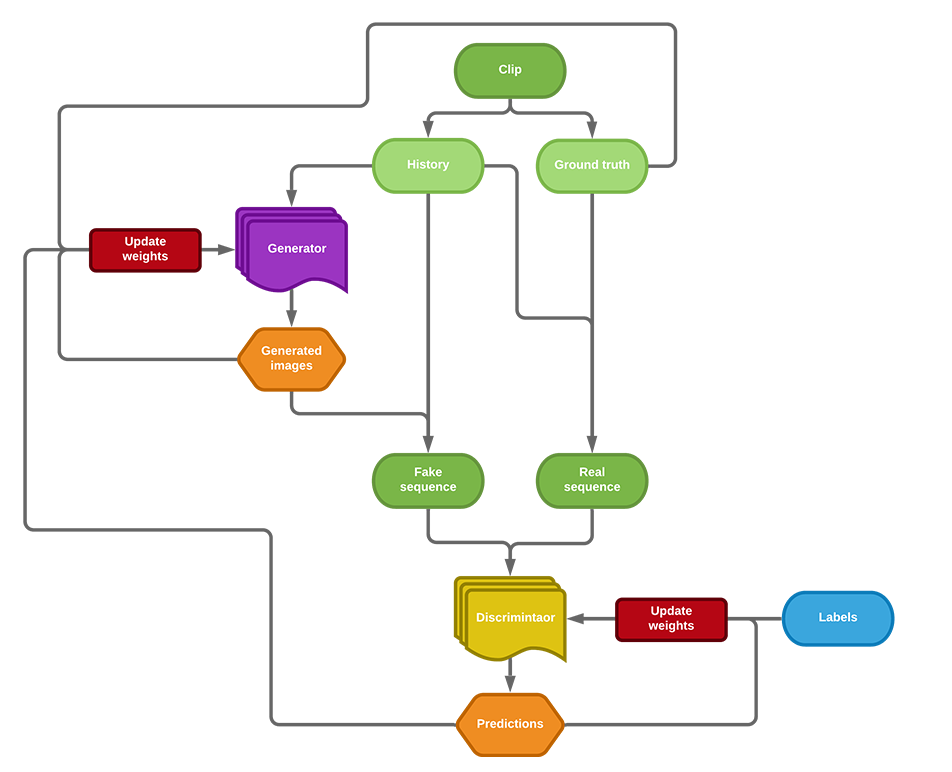
\includegraphics[width=0.7\linewidth]{gan-graph.png}
\end{figure}

\clearpage

In this model, the generator and discriminator are both multi-scale models \cite{multiscale}.

The discriminator is a convolutional neural network image classifier that runs the clips through convolutional layers activated with ReLU (rectified linear unit), and then to fully connected layers to obtain a scalar prediction between 0 and 1. It operates on a multi-scale model, meaning that a 64 by 64 pixel square clip is downscaled to 8 by 8, 16 by 16, 32 by 32, and the original clip, and a prediction generated for each scale.

The generator is a fully convolutional image generator model that also operates with the same four-scale model. However, a significant difference from the discriminator is that the generator concatenates the upsampled output of each scale to the next one to strengthen the time dependency.

\begin{figure}[H]
    \caption{graph of the discriminator and generator models}
    \centering
    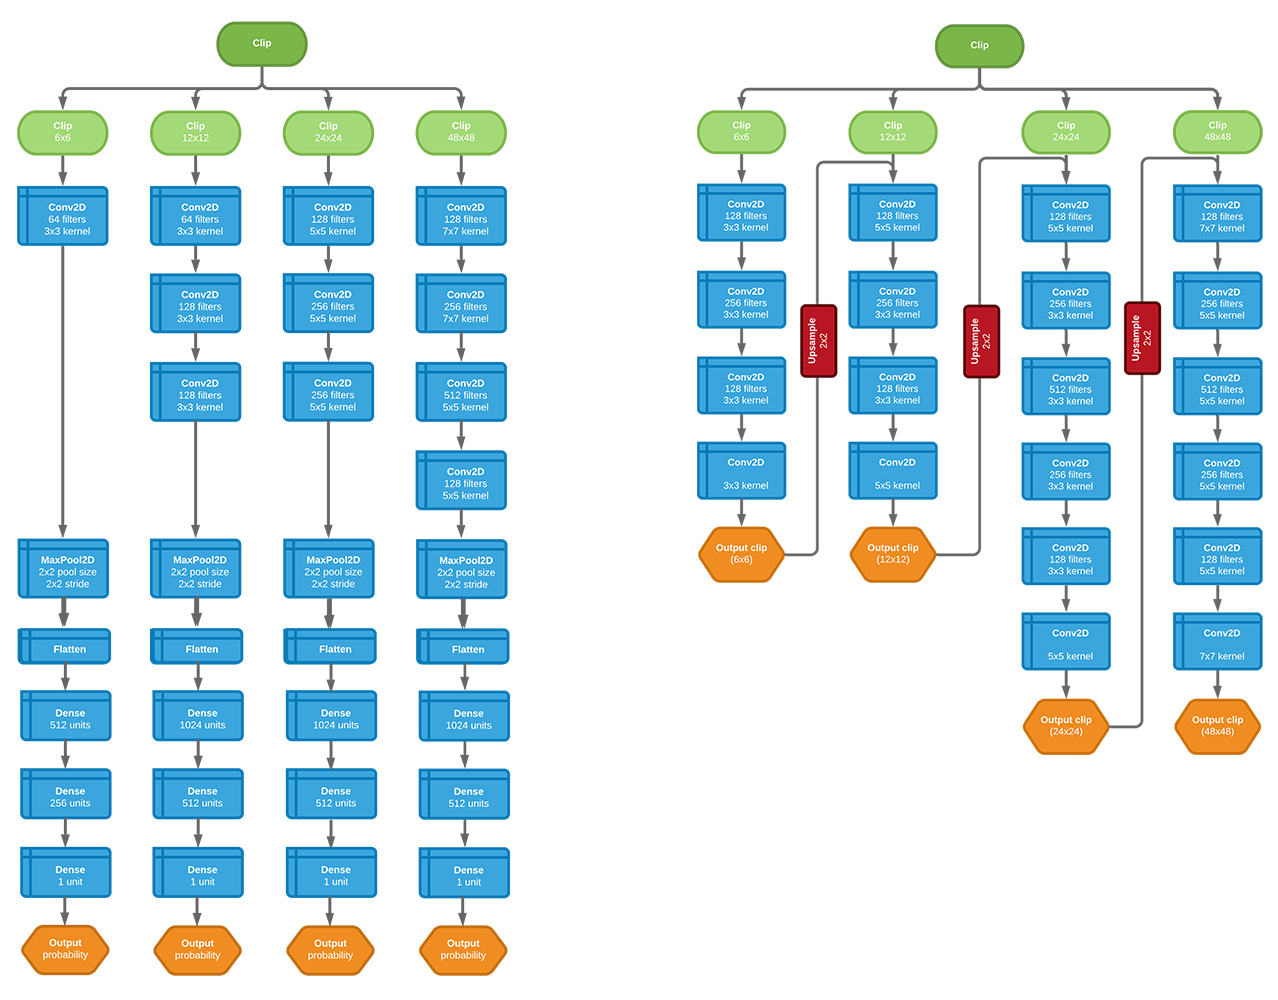
\includegraphics[width=1.0\linewidth]{disc-gen-graph.png}
\end{figure}

\clearpage

\subsection{Data preprocessing}

Before being fed to the model, the satellite images need to be preprocessed for compatibility, efficiency, and enhancement.

\subsection*{Clip stacking}

The first element of preprocessing is in stacking a series of time-ordered into a single "clip" unit that can be passed to the model as one object. In this model, clips were treated as either sequences of individual frames sequenced into a list, or as a single three-dimensional matrix of shape,
\begin{align*}
    (\textrm{height}, \textrm{width}, \textrm{number of frames}
    \times \textrm{number of channels})
\end{align*}

Essentially, a stacked clip of two RGB images would be visualized as such,

\begin{figure}[H]
    \centering
    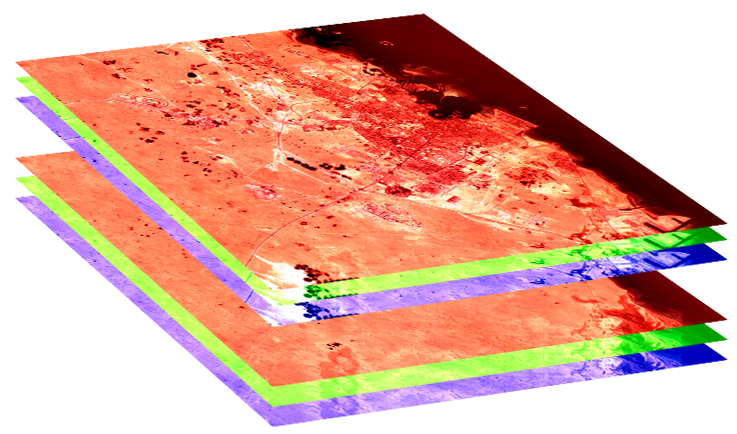
\includegraphics[width=0.5\linewidth]{clip-stack.png}
\end{figure}

\subsection*{Clip cropping}

Due to memory constraints, as well as ease of upsampling and downsampling images for the sake of the multi-scale model, the images are cropped into 64 $\times$ 64 squares. Since the generator is purely convolutional, it can actually generate images of any size using weights trained on smaller squares, which is why this model is able to generate full-sized maps.

\subsection*{Filter enhancement}

In order to help the model recognize the urbanized areas more clearly, contrast and brightness filters were applied in image preprocessing to make urban areas more distinct compared to the surrounding desert. A satellite map with the filters applied would appear as such,

\begin{figure}[H]
    \centering
    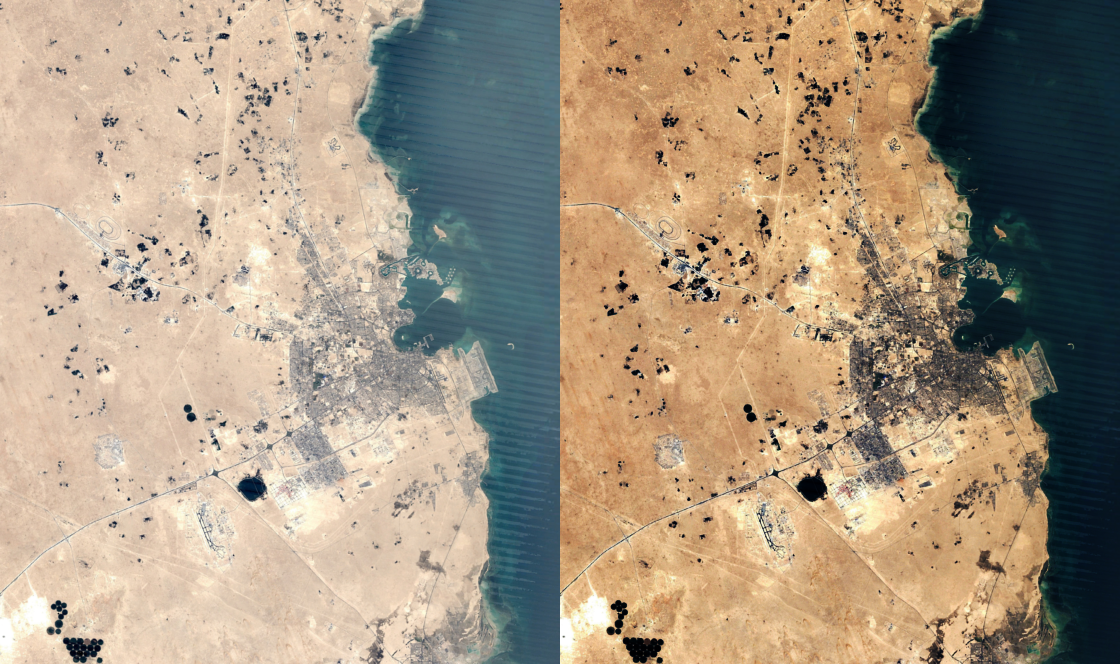
\includegraphics[width=0.7\linewidth]{enhanced-comp.png}
\end{figure}

\clearpage

\subsection{Loss functions}

To mathematically define the loss functions used in training, we must first define the generator and discriminator models as functions,
\begin{align*}
    \mathrm{gen} &: \textrm{ images } \to \textrm{ images }\\
    \mathrm{disc} &: \textrm{ images } \to [0, 1]
\end{align*}

\subsection*{$\ell_p$ loss}

We define the $\ell_p$ loss as,
\begin{align*}
    \ell_p(x, y) = |x - y|^p,\; p \in \big\{1, 2\big\}
\end{align*}

This loss represents either the absolute difference (if $p = 1$), or the absolute squared difference (if $p = 2$) between the generated images $x$ and the ground truth images $y$. This is the simplest metric for the accuracy of the generated images.

\subsection*{Adversarial loss}

First, define the binary crossentropy loss as,
\begin{align*}
    \mathrm{bce}(y, y') = -\sum_i y_i\log(y_i') + (1-y_i)
    \log(1-y_i')
\end{align*}

where $y$ represents the predicted labels given as output of the discriminator, and $y'$ represents the true labels assigned to the data. For each generate image that the discriminator receives, it generates a probability that this image matches the ground truth image. The binary crossentropy loss is a measure of how close this probability is to the truth. It operates on a logarithmic basis, so probabilities that are the same as the true label have a very small loss, while probabilities that are very far from the true label have an enormous loss.

Next, we define the discriminator loss,
\begin{align*}
    \mathrm{loss}_{\mathrm{disc}}(x, y) =
    \mathrm{bce}(\mathrm{disc}(x, y), 1) +
    \mathrm{bce}(\mathrm{disc}(x, \mathrm{gen}(x)), 0)
\end{align*}

\subsection*{Discriminator loss}

The loss used for the discriminator is defined as,
\begin{align*}
    \mathrm{adv}(x, y) =
    \mathrm{bce}(\mathrm{disc}(x, \mathrm{gen}(x)), 0)
\end{align*}

\subsection*{Gradient difference loss (GDL)}

Define the image GDL \cite{multiscale} as,
\begin{align*}
    \mathrm{gdl}(x, y) = \sum_{i, j}\left||y_{i, j} - y_{i - 1, j}| -
    |\mathrm{gen}(x)_{i, j} - \mathrm{gen}(x)_{i - 1, j}|\right|^c\\
    + \left||y_{i, j - 1} - y_{i, j}| -
    |\mathrm{gen}(x)_{i, j - 1} - \mathrm{gen}(x)_{i, j}|\right|^c
\end{align*}

This is used to penalize images that are significantly blurry and fuzzy, to improve definition of the final predicted image. The value of $c$ is a constant to be determined through arbitrary choice or fine tuning. For the purposes of the \texttt{dohamaps} model, the value of $c = 1$ was used.

\subsection*{Generator loss (combined)}

Finally, the combined loss, which is used as the loss for the generator,
\begin{align*}
    \mathrm{loss}_{\mathrm{gen}}(x, y) = \alpha\, \mathrm{adv}(x, y) +
    \beta\, \mathrm{\ell}_p(x, y) + \gamma\, \mathrm{gdl}(x, y)
\end{align*}

Once again, the values of $\alpha,$ $\beta,$ and $\gamma$ are constants, which in the \texttt{dohamaps} model were set to $\alpha = 0.05,$ $\beta = 1,$ and $\gamma = 1$.

\clearpage

\subsection{Metrics}

In addition to the loss functions, the model contains metrics. These metrics do not directly inform the training loop, but are reported regularly to provide measures of the model's performance.

\subsection*{Peak signal to noise ratio (PSNR)}

The PSNR is defined as,
\begin{align*}
    \mathrm{psnr}(x, y) = 10 \cdot \log_{10}\left( \frac{N \cdot
    \mathrm{max}}{\sum (x_i - y_i)} \right)
\end{align*}

where $N$ is the number of channels, and $\mathrm{max}$ is the maximum value of the image signal. In a default RGB image, this value is 255. The PSNR is measured in decibels, where a higher value indicates an image that is harder to distinguish from the original by the naked eye. We are aiming for a high PSNR. 

\subsection*{Sharpness difference}

The sharpness difference is defined as,
\begin{align*}
    \mathrm{sharpdiff}(x, y) = 10 \cdot \log_{10}\left(\frac{N \cdot
    \mathrm{max}^2}{\sum_i \sum_j |(\Delta_i x + \Delta_j x) - (\Delta_i
    y + \Delta_j y)|}\right)
\end{align*}

which measures the loss of sharpness between the true frame $x$ and the predicted image $y$. Ideally, we are aiming for a very low sharpness difference.

\subsection*{Structural similarity index measure (SSIM)}

Define the SSIM \cite{ssim} as,
\begin{align*}
    \mathrm{ssim}(x, y) = \frac{(2\mu_x\mu_y + c_1)(2\sigma_{xy} + c_2)}
    {(\mu_x^2 + \mu_y^2 + c_1)(\sigma_x^2 + \sigma_y^2 + c_2)}
\end{align*}

where $\mu_x$ is the average of image $x$, and $\mu_y$ is the average of image $y$, $\sigma_x$ and $\sigma_y$ are the variance of $x$ and $y$, $\sigma_{xy}$ is the covariance of $x$ and $y$, and $c_1$ and $c_2$ are constants. We are aiming for an SSIM value that is as close to 1 as possible. 

\clearpage

\subsection{Hyperparameters}

In addition to the losses and metrics defined above, there are several significant hyperparameters that can heavily influence the training and outputs of the model. The generator and the discriminator both use the Adam optimizer \cite{adam}, which has takes as its main parameter the learning rate. Learning rates that are too high will cause the loss to oscillate and lead to inaccurate results, while learning rates that are too low will not converge in a reasonable amount of time.

The next pair of hyperparameters are the history and prediction length. The history length represents the length of the clip taken as an input to the generator, while the prediction length represents the length of the clip output as a prediction. Predictions beyond the length of the prediction clip are computed recursively from initial prediction. Image sequences that change over time, but not necessarily in a strongly time-linked pattern, benefit from a shorter history and prediction length. For the purposes of urban growth, where time-linked patterns are important, longer history and prediction lengths are beneficial.

The final hyperparameter is a combination of two items:
\begin{enumerate}[label=(\alph*)]
    \item The size of the clips are preprocessed from the input images.
    \item The scale of the images that the clips are sourced from.
\end{enumerate}

The significance of this is in the ratio between the two. Reducing overall image size and increasing the size of the clips allows capturing more large-scale features at the cost of detail and small-scale definition, while the inverse would lead to very high definition images that miss large time-dependent features.

\clearpage

\section{Testing and tuning}

Tuning hyperparameters and model architecture is a matter of trial and error. As such, numerous trial runs were conducted with various values of the hyperparameters. This section will discuss the most significant trials.

\subsection{Exhibit A}

\begin{table}[h]
\begin{tabular}{ll}
\textbf{Hyperparameter} & \textbf{Value}\\
Generator learning rate & 0.00004\\
Discriminator learning rate & 0.00002\\
History length & 4 frames\\
Prediction length & 1 frames\\
Clip size & 32 $\times$ 32\\
Image size & 2800 $\times$ 3320\\
\end{tabular}
\end{table}

\begin{figure}[H]
    \caption{2020 (left) vs. generated 2035 (right)}
    \centering
    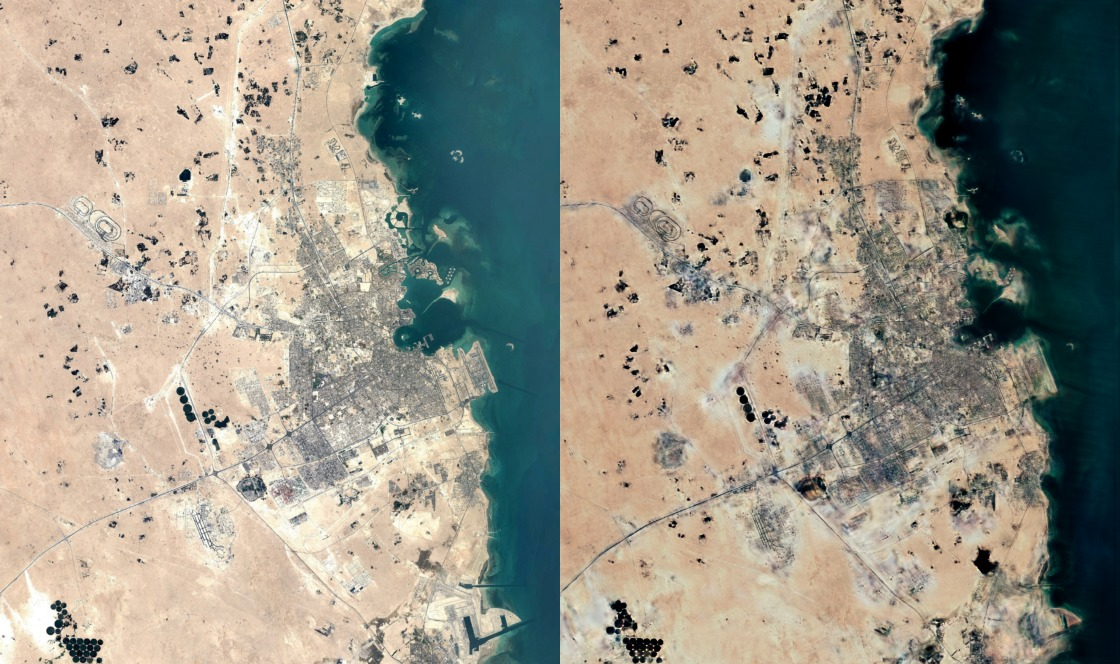
\includegraphics[width=0.7\linewidth]{exhibit-a-comp.jpg}
\end{figure}

In comparison to the goals of the model stated in the introduction, this output meets two of the three objectives decently well.

\begin{enumerate}[label=(\alph*)]
    \item It displays a viable image of a simulated Doha that looks reasonable and believable. It lacks some definition in certain areas and has artifacts from the enhancement filters applied in the training, however looking at it clearly resembles a real-life map of Doha.
    \item It preserves the coastline extremely well, with essentially no changes to it, including the airport and the Pearl areas.
\end{enumerate}

\clearpage

\subsection{Exhibit B}

\begin{table}[h]
\begin{tabular}{ll}
\textbf{Hyperparameter} & \textbf{Value}\\
Generator learning rate & 0.000005\\
Discriminator learning rate & 0.00002\\
History length & 8 frames\\
Prediction length & 8 frames\\
Clip size & 48 $\times$ 48\\
Image size & 560 $\times$ 664\\
\end{tabular}
\end{table}

\begin{figure}[H]
    \caption{2020 (left) vs. generated 2035 (right)}
    \centering
    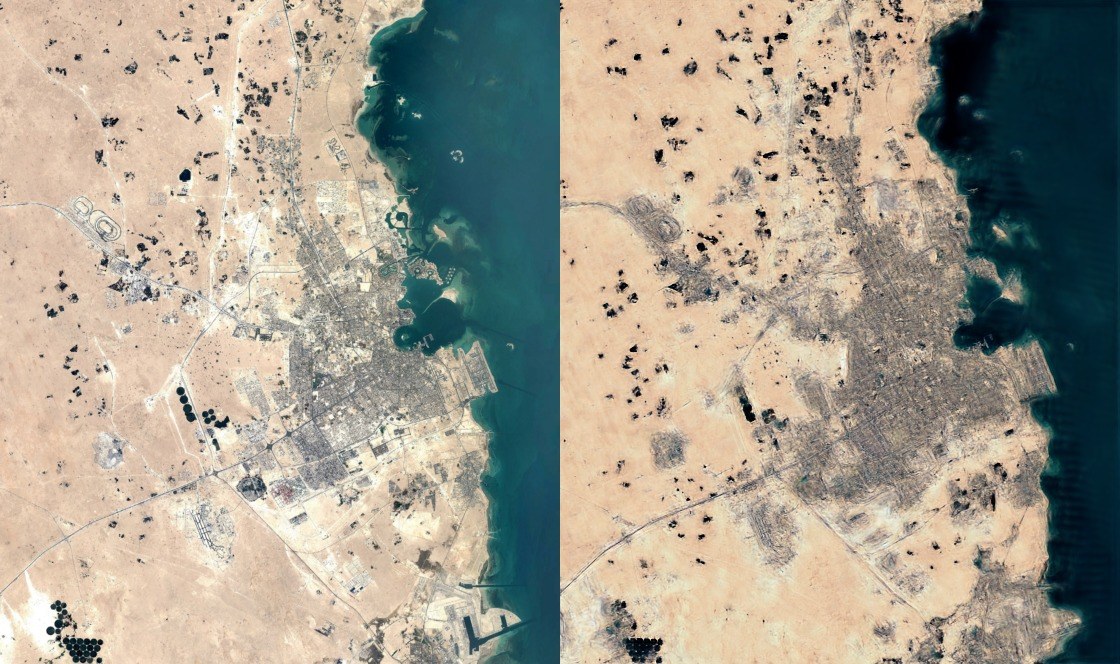
\includegraphics[width=0.7\linewidth]{exhibit-b-comp.jpg}
\end{figure}

This model improves in some areas compared to the stated goals, although it still needs some work.

\begin{enumerate}[label=(\alph*)]
    \item It displays a viable image of a simulated Doha that looks somewhat reasonable and believable. It lacks a lot of definition, even compared to Exhibit A's output, however, it still resembles Doha.
    \item It preserves the coastline decently well, with mostly no changes, although some areas near the southern end of the coastline are blurry or altered.
\end{enumerate}

\clearpage

\subsection{Exhibit C}

\begin{table}[h]
\begin{tabular}{ll}
\textbf{Hyperparameter} & \textbf{Value}\\
Generator learning rate & 0.00000085\\
Discriminator learning rate & 0.000005\\
History length & 11 frames\\
Prediction length & 19 frames\\
Clip size & 64 $\times$ 64\\
Image size & 560 $\times$ 664\\
\end{tabular}
\end{table}

\begin{figure}[H]
    \caption{2020 (left) vs. generated 2035 (right)}
    \centering
    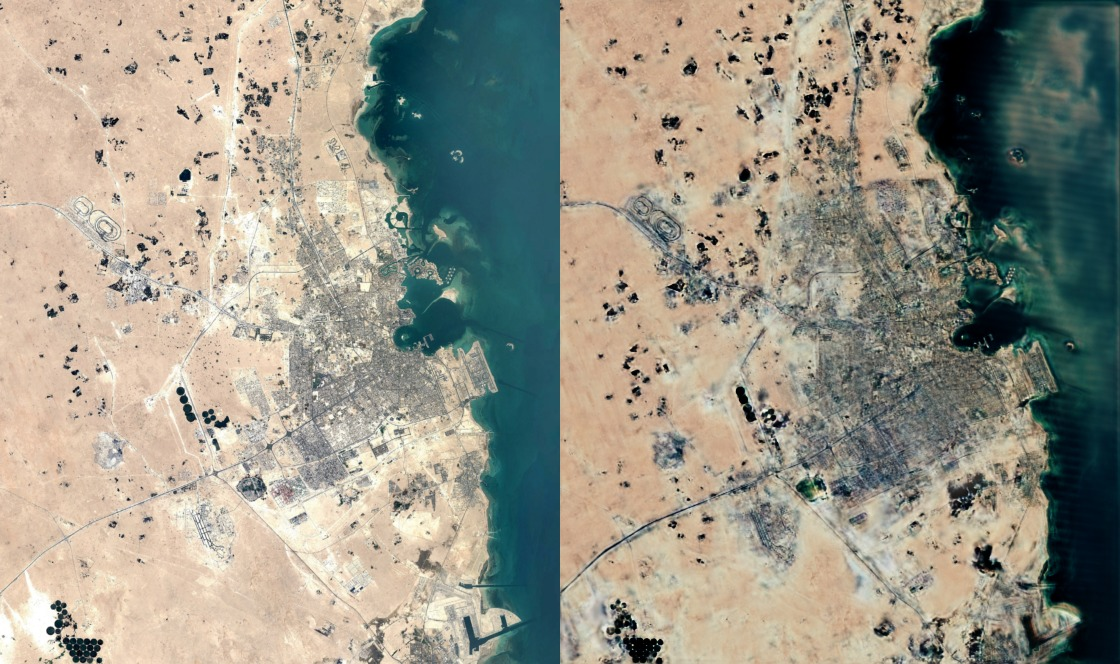
\includegraphics[width=0.7\linewidth]{exhibit-c-comp.jpg}
\end{figure}

In comparison to the goals of the model stated in the introduction, this output meets all of the three objectives decently well.

\begin{enumerate}[label=(\alph*)]
    \item It displays a viable image of a simulated Doha that looks quite reasonable and believable. It lacks the extreme fine-detail definition of Exhibit A, however it preserves most features such as roads and specific clusters of buildings that were already present in the city.
    \item It preserves the coastline well, with virtually no changes.
\end{enumerate}

\clearpage

\begin{thebibliography}{9}
\bibitem{goodfellow}
Ian J. Goodfellow, Jean Pouget-Abadie, Mehdi Mirza, Bing Xu, David Warde-Farley, Sherjil Ozair, Aaron C. Courville, and Yoshua Bengio. Generative adversarial networks. NIPS, 2014.

\bibitem{ssim}
Wang, Zhou, Bovik, Alan C., Sheikh, Hamid R., and Simoncelli, Eero P. Image quality assessment: From error visibility to structural similarity. \textit{IEEE Trans. on Im. Proc.}, 13(4):600–612, 2004.

\bibitem{adam}
Diederik P. Kingma, and Jimmy Ba, Adam: A Method for Stochastic Optimization, 2014.

\bibitem{multiscale}
Michael Mathieu, Camille Couprie, and Yann LeCun, Deep multi-scale video prediction beyond mean square error, 2015.

\end{thebibliography}

\end{document}
